\pdfminorversion=4 % for acroread
\documentclass[t]{beamer}
%\documentclass[t,handout]{beamer}

\usepackage[english]{babel}
\usepackage[utf8]{inputenc}
\usepackage{graphicx}

\usepackage{amsmath,amssymb}
\usepackage{listings}
\lstset{frame=lines,framesep=3pt,numbers=left,numberblanklines=false,basicstyle=\ttfamily\small}

\usepackage{subfig}
\usepackage{multicol}
\usepackage{appendixnumberbeamer}

\usepackage{tikz}
\usetikzlibrary{trees} 
\usetikzlibrary{shapes.geometric}
\usetikzlibrary{positioning,shapes,shadows,arrows,calc,mindmap}
\pgfdeclarelayer{background}
\pgfdeclarelayer{foreground}
\pgfsetlayers{background,main,foreground}
\tikzstyle{activity}=[rectangle, draw=white, rounded corners, text centered, text width=8em]
\tikzstyle{data}=[rectangle, draw=white, text centered, text width=8em]
\tikzstyle{myarrow}=[->, thick, draw=white]

% Define the layers to draw the diagram
\pgfdeclarelayer{background}
\pgfdeclarelayer{foreground}
\pgfsetlayers{background,main,foreground}


\usepackage{listings}
\lstset{numbers=left,
  showstringspaces=false,
  frame={tb},
  captionpos=b,
  lineskip=0pt,
  basicstyle=\ttfamily,
  extendedchars=true,
  stepnumber=1,
  numberstyle=\small,
  xleftmargin=1em,
  breaklines
}

\renewcommand{\comment}[1]{
	\noindent
	%\vspace{0.25cm}
	{\color{red}{\textbf{TODO:} #1}}
	%\vspace{0.25cm}
}
\newcommand{\notefh}[1]{\textcolor{red}{\textbf{FH:} #1}}
\renewcommand{\comment}[1]{}
\newcommand{\hide}[1]{}
\newcommand{\cemph}[2]{\emph{\textcolor{#1}{#2}}}

\newcommand{\lit}[1]{{\footnotesize\color{black!60}[#1]}}

\newcommand{\litw}[1]{{\footnotesize\color{blue!20}[#1]}}


\newcommand{\myframe}[2]{\begin{frame}[c]{#1}#2\end{frame}}
\newcommand{\myframetop}[2]{\begin{frame}{#1}#2\end{frame}}
\newcommand{\myit}[1]{\begin{itemize}#1\end{itemize}}
\newcommand{\myblock}[2]{\begin{block}{#1}#2\end{block}}


\newcommand{\votepurple}[1]{\textcolor{Purple}{$\bigstar$}}
\newcommand{\voteyellow}[1]{\textcolor{Goldenrod}{$\bigstar$}}
\newcommand{\voteblue}[1]{\textcolor{RoyalBlue}{$\bigstar$}}
\newcommand{\votepink}[1]{\textcolor{Pink}{$\bigstar$}}

\newcommand{\diff}{\mathop{}\!\mathrm{d}}
\newcommand{\refstyle}[1]{{\small{\textcolor{gray}{#1}}}}
\newcommand{\hands}[0]{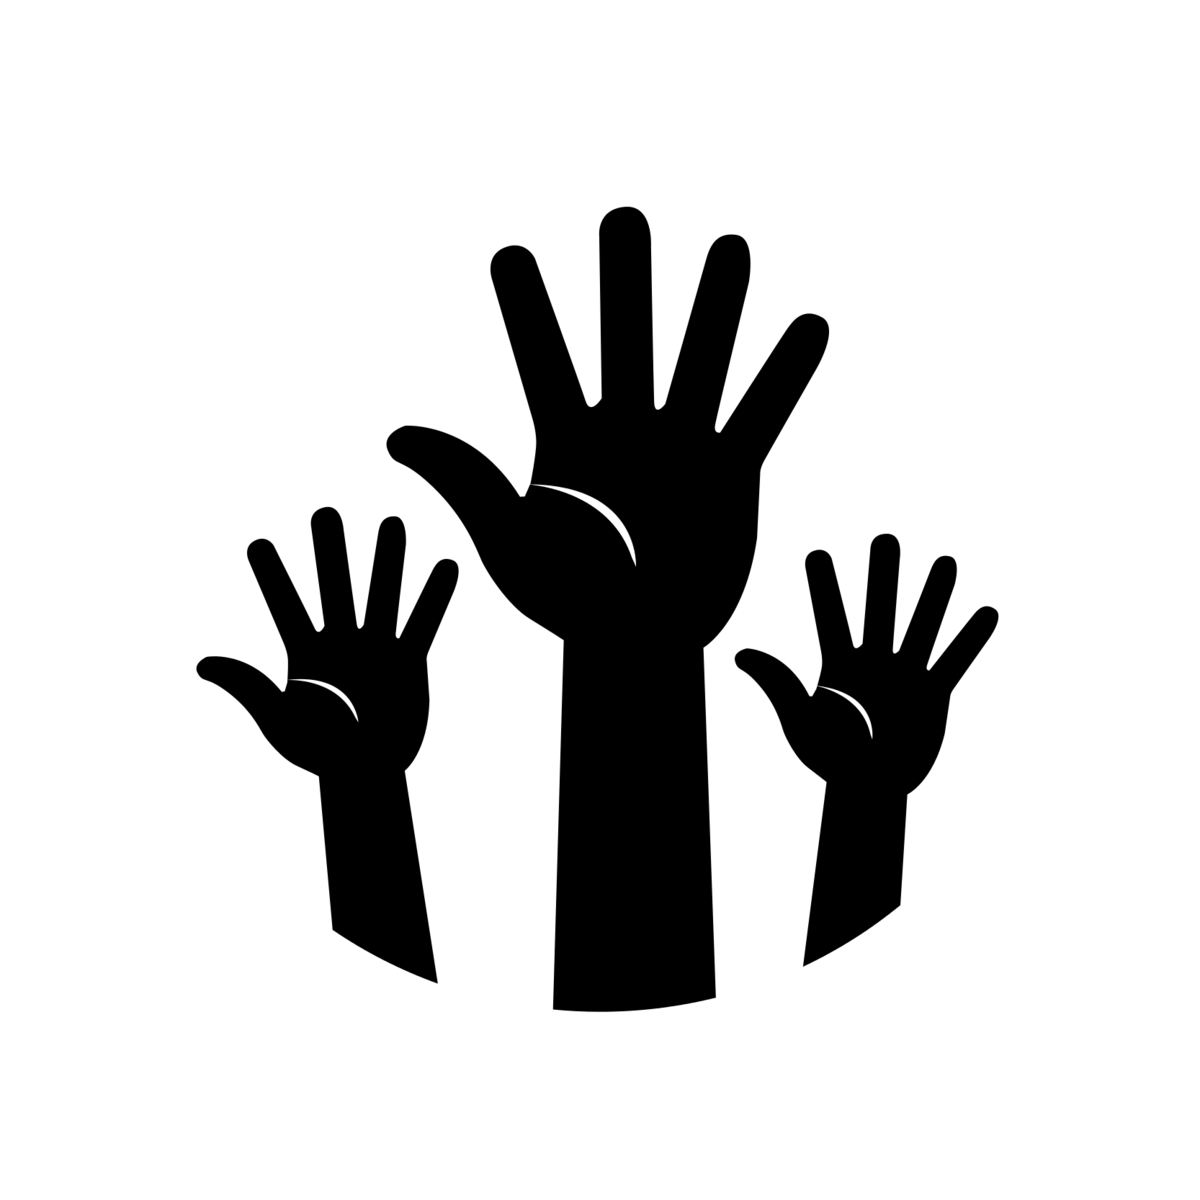
\includegraphics[height=1.5em]{images/hands}}
\newcommand{\transpose}[0]{{\textrm{\tiny{\sf{T}}}}}
\newcommand{\norm}{{\mathcal{N}}}
\newcommand{\cutoff}[0]{\kappa}
\newcommand{\instD}[0]{\dataset}
\newcommand{\insts}[0]{\mathcal{I}}
\newcommand{\inst}[0]{i}
\newcommand{\instI}[1]{i^{(#1)}}

% Iteration specific instance of variable/function/anything
% Introduced in the BO section, but moved up here to make it available within other macros
\newcommand{\iter}[2][\bocount]{{#2}^{(#1)}}

%--------HPO parameter macros-----------

% Parameter Configuration Space
\newcommand{\pcs}[0]{\pmb{\Lambda}}

% ???
\newcommand{\bx}[0]{\conf}

% Parameter Configuration
\newcommand{\conf}[0]{\pmb{\lambda}}

% Final Configuration
\newcommand{\finconf}[0]{\pmb{\hat{\lambda}}}

% Configuration corresponding to a given iteration -- better use \iter!
\newcommand{\confI}[1]{{\conf}^{(#1)}}

% Default Configuration
\newcommand{\defconf}[0]{{\conf}_{\text{def}}}

% Incumbent Configuration
\newcommand{\incumbent}[1][\bocount]{\iter[#1]{\finconf}}

% Optimal Configuration
\newcommand{\optconf}[0]{{\conf}^*}

% Configuration Space
\newcommand{\confs}[0]{\pcs}

%----------------------------------------

%\newcommand{\vlambda}[0]{\bm{\lambda}}
%\newcommand{\vLambda}[0]{\bm{\Lambda}}
\newcommand{\dataset}[0]{\mathcal{D}}
\newcommand{\datasets}[0]{\mathbf{D}}
\newcommand{\loss}[0]{L}
\newcommand{\risk}{\mathcal{R}}
\newcommand{\riske}{\mathcal{R}_{\text{emp}}}
\newcommand{\cost}[0]{c}
\newcommand{\costI}[1]{c^{(#1)}}

% Gaussian Process
\newcommand{\gp}{\mathcal{G}}
% Family of Objective Functions
\newcommand{\objF}{F}

%---------------BO Macros------------------

% BO loop counter
\newcommand{\bocount}{t}
% BO loop counter max, the counter runs from 1 to this value
\newcommand{\bobudget}{T}
% BO loop observation
\newcommand{\obs}[1][\conf]{\cost({#1})}
% BO loop observation space
\newcommand{\obsspace}{\mathcal{Y}}
% BO loop next observation
\newcommand{\bonextobs}{\obs[\iter{\conf}]}
% Acquisition Function, no args
\newcommand{\acq}{u}
% Standard Normal PDF
\newcommand{\pdf}{\phi}
% Standard Normal CDF
\newcommand{\cdf}{\Phi}
% Mean
\newcommand{\mean}{\mu}
% Standard Deviation
\newcommand{\stddev}{\sigma}
% Variance
\newcommand{\variance}{\sigma^2}
% Noise
\newcommand{\noise}{\nu}
% BO loop next selected sample
\newcommand{\bonextsample}{\confI{\bocount}}

% Single hyperparameter
\newcommand{\hyperparam}{\lambda}

% Single hyperparameter within a hyperparameter configuration
\newcommand{\hyperparami}[1][i]{{\hyperparam}_#1}

% Full definition of final configuration
\newcommand{\finconffull}{\incumbent[\bobudget]}

% Dataset
\newcommand{\datasetHPO}{{\dataset}_{HPO}}

% Dataset definition
\newcommand{\datasetHPOdef}{{\langle \bonextsample,\,\bonextobs \rangle}_{\bocount=1}^{\bobudget}}

% Double Display Fraction, forces large displays for everything in numerator and denominator
\newcommand\ddfrac[2]{\frac{\displaystyle #1}{\displaystyle #2}}

% Conditional Probability "Given That" Relation, source:https://tex.stackexchange.com/a/141685/205886
\newcommand\given[1][]{\:#1\vert\:}

% Expectation as a math operator
\DeclareMathOperator*{\E}{\mathbb{E}}

% Citation 
\newcommand{\source}[1]{
    \begin{flushright}
    	Source: \lit{#1}
    \end{flushright}
}
%-------------------------------------------

%Real numbers set
\newcommand{\realnum}{\mathbb{R}}
%Configuration space - do not use
%\newcommand{\configspace}{\Theta}
%Instances - do not use
%\newcommand{\instances}{\mathcal{I}}
%Expected value
\newcommand{\expectation}{\mathbb{E}}
%Kernel
\newcommand{\kernel}{\kappa}
%Constraint function
\newcommand{\constraintf}{c}
%Normal distribution
\newcommand{\normaldist}{\mathcal{N}}

% \renewcommand{\vec}[1]{\mathbf{#1}}
\newcommand{\hist}[0]{\dataset_{\text{Hist}}}
\newcommand{\param}[0]{p}
\newcommand{\algo}[0]{\mathcal{A}}
\newcommand{\algos}[0]{\mathbf{A}}
%\newcommand{\nn}[0]{N}
\newcommand{\feats}[0]{\mathcal{X}_{\text{meta}}}
\newcommand{\feat}[0]{\x_{\text{meta}}}
%\newcommand{\cluster}[0]{\vec{h}}
%\newcommand{\clusters}[0]{\vec{H}}
\newcommand{\perf}[0]{\mathbb{R}}
%\newcommand{\surro}[0]{\mathcal{S}}
\newcommand{\surro}[0]{\hat{\cost}}
\newcommand{\func}[0]{f}
\newcommand{\epm}[0]{\surro}
\newcommand{\portfolio}[0]{\mathbf{P}}
\newcommand{\schedule}[0]{\mathcal{S}}

% Machine Learning
\newcommand{\mdata}[0]{\dataset_{\text{meta}}}
\newcommand{\datasettrain}[0]{\dataset_{\text{train}}}
\newcommand{\datasetval}[0]{\dataset_{\text{val}}}
\newcommand{\datasettest}[0]{\dataset_{\text{test}}}
\newcommand{\x}[0]{\mathbf{x}}
\newcommand{\y}[0]{y}
\newcommand{\xI}[1]{\mathbf{x}^{(#1)}}
\newcommand{\yI}[1]{y^{(#1)}}
\newcommand{\fx}{f(\mathbf{x})}  % f(x), continuous prediction function
\newcommand{\Hspace}{\mathcal{H}} % hypothesis space where f is from
\newcommand{\fh}{\hat{f}}       % f hat, estimated prediction function

% Deep Learning
\newcommand{\weights}[0]{\theta}
\newcommand{\metaweights}[0]{\phi}


% reinforcement learning
\newcommand{\policies}[0]{\mathbf{\Pi}}
\newcommand{\policy}[0]{\pi}
\newcommand{\actionRL}[0]{a}
\newcommand{\stateRL}[0]{s}
\newcommand{\statesRL}[0]{\mathcal{S}}
\newcommand{\rewardRL}[0]{r}
\newcommand{\rewardfuncRL}[0]{\mathcal{R}}

\RestyleAlgo{algoruled}
\DontPrintSemicolon
\LinesNumbered
\SetAlgoVlined
\SetFuncSty{textsc}

\SetKwInOut{Input}{Input}
\SetKwInOut{Output}{Output}
\SetKw{Return}{return}

%\newcommand{\changed}[1]{{\color{red}#1}}

%\newcommand{\citeN}[1]{\citeauthor{#1}~(\citeyear{#1})}

\renewcommand{\vec}[1]{\mathbf{#1}}
\DeclareMathOperator*{\argmin}{arg\,min}
\DeclareMathOperator*{\argmax}{arg\,max}

%\newcommand{\aqme}{\textit{AQME}}
%\newcommand{\aslib}{\textit{ASlib}}
%\newcommand{\llama}{\textit{LLAMA}}
%\newcommand{\satzilla}{\textit{SATzilla}}
%\newcommand{\satzillaY}[1]{\textit{SATzilla'{#1}}}
%\newcommand{\snnap}{\textit{SNNAP}}
%\newcommand{\claspfolioTwo}{\textit{claspfolio~2}}
%\newcommand{\flexfolio}{\textit{FlexFolio}}
%\newcommand{\claspfolioOne}{\textit{claspfolio~1}}
%\newcommand{\isac}{\textit{ISAC}}
%\newcommand{\eisac}{\textit{EISAC}}
%\newcommand{\sss}{\textit{3S}}
%\newcommand{\sunny}{\textit{Sunny}}
%\newcommand{\ssspar}{\textit{3Spar}}
%\newcommand{\cshc}{\textit{CSHC}}
%\newcommand{\cshcpar}{\textit{CSHCpar}}
%\newcommand{\measp}{\textit{ME-ASP}}
%\newcommand{\aspeed}{\textit{aspeed}}
%\newcommand{\autofolio}{\textit{AutoFolio}}
%\newcommand{\cedalion}{\textit{Cedalion}}
\newcommand{\fanova}{\textit{fANOVA}}
\newcommand{\sbs}{\textit{SB}}
\newcommand{\oracle}{\textit{VBS}}

% like approaches
\newcommand{\claspfoliolike}[1]{\texttt{claspfolio-#1-like}}
\newcommand{\satzillalike}[1]{\texttt{SATzilla'#1-like}}
\newcommand{\isaclike}{\texttt{ISAC-like}}
\newcommand{\ssslike}{\texttt{3S-like}}
\newcommand{\measplike}{\texttt{ME-ASP-like}}

\newcommand{\irace}{\textit{I/F-race}}
\newcommand{\gga}{\textit{GGA}}
\newcommand{\smac}{\textit{SMAC}}
\newcommand{\paramils}{\textit{ParamILS}}
\newcommand{\spearmint}{\textit{Spearmint}}
\newcommand{\tpe}{\textit{TPE}}


\usepackage{pifont}
\newcommand{\itarrow}{\mbox{\Pisymbol{pzd}{229}}}
\newcommand{\ithook}{\mbox{\Pisymbol{pzd}{52}}}
\newcommand{\itcross}{\mbox{\Pisymbol{pzd}{56}}}
\newcommand{\ithand}{\mbox{\raisebox{-1pt}{\Pisymbol{pzd}{43}}}}

%\DeclareMathOperator*{\argmax}{arg\,max}

\newcommand{\ie}{{\it{}i.e.\/}}
\newcommand{\eg}{{\it{}e.g.\/}}
\newcommand{\cf}{{\it{}cf.\/}}
\newcommand{\wrt}{\mbox{w.r.t.}}
\newcommand{\vs}{{\it{}vs\/}}
\newcommand{\vsp}{{\it{}vs\/}}
\newcommand{\etc}{{\copyedit{etc.}}}
\newcommand{\etal}{{\it{}et al.\/}}

\newcommand{\pscProc}{{\bf procedure}}
\newcommand{\pscBegin}{{\bf begin}}
\newcommand{\pscEnd}{{\bf end}}
\newcommand{\pscEndIf}{{\bf endif}}
\newcommand{\pscFor}{{\bf for}}
\newcommand{\pscEach}{{\bf each}}
\newcommand{\pscThen}{{\bf then}}
\newcommand{\pscElse}{{\bf else}}
\newcommand{\pscWhile}{{\bf while}}
\newcommand{\pscIf}{{\bf if}}
\newcommand{\pscRepeat}{{\bf repeat}}
\newcommand{\pscUntil}{{\bf until}}
\newcommand{\pscWithProb}{{\bf with probability}}
\newcommand{\pscOtherwise}{{\bf otherwise}}
\newcommand{\pscDo}{{\bf do}}
\newcommand{\pscTo}{{\bf to}}
\newcommand{\pscOr}{{\bf or}}
\newcommand{\pscAnd}{{\bf and}}
\newcommand{\pscNot}{{\bf not}}
\newcommand{\pscFalse}{{\bf false}}
\newcommand{\pscEachElOf}{{\bf each element of}}
\newcommand{\pscReturn}{{\bf return}}

%\newcommand{\param}[1]{{\sl{}#1}}
\newcommand{\var}[1]{{\it{}#1}}
\newcommand{\cond}[1]{{\sf{}#1}}
%\newcommand{\state}[1]{{\sf{}#1}}
%\newcommand{\func}[1]{{\sl{}#1}}
\newcommand{\set}[1]{{\Bbb #1}}
%\newcommand{\inst}[1]{{\tt{}#1}}
\newcommand{\myurl}[1]{{\small\sf #1}}

\newcommand{\Nats}{{\Bbb N}}
\newcommand{\Reals}{{\Bbb R}}
\newcommand{\extset}[2]{\{#1 \; | \; #2\}}

\newcommand{\vbar}{$\,\;|$\hspace*{-1em}\raisebox{-0.3mm}{$\,\;\;|$}}
\newcommand{\vendbar}{\raisebox{+0.4mm}{$\,\;|$}}
\newcommand{\vend}{$\,\:\lfloor$}


\newcommand{\goleft}[2][.7]{\parbox[t]{#1\linewidth}{\strut\raggedright #2\strut}}
\newcommand{\rightimage}[2][.3]{\mbox{}\hfill\raisebox{1em-\height}[0pt][0pt]{\includegraphics[width=#1\linewidth]{#2}}\vspace*{-\baselineskip}}
 

\usetheme{Madrid}
\useinnertheme{rectangles}
\usecolortheme{whale}
\setbeamercolor{alerted text}{fg=blue}
\useoutertheme{infolines}
\setbeamertemplate{navigation symbols}{\vspace{-5pt}} % to lower the logo
\setbeamercovered{invisible}

\makeatletter
\setbeamertemplate{footline}
{
  \leavevmode%
  \hbox{%
  \begin{beamercolorbox}[wd=.333333\paperwidth,ht=2.25ex,dp=1ex,center]{author in head/foot}%
    \usebeamerfont{author in head/foot}\insertshortauthor
  \end{beamercolorbox}%
  \begin{beamercolorbox}[wd=.333333\paperwidth,ht=2.25ex,dp=1ex,center]{title in head/foot}%
    \usebeamerfont{title in head/foot}\insertshorttitle
  \end{beamercolorbox}%
  \begin{beamercolorbox}[wd=.333333\paperwidth,ht=2.25ex,dp=1ex,right]{date in head/foot}%
    \usebeamerfont{date in head/foot}\insertshortdate{}\hspace*{2em}
    \insertframenumber\hspace*{2ex} 
  \end{beamercolorbox}}%
  \vskip0pt%
}
\makeatother

\newcommand{\lit}[1]{{\footnotesize\color{black!70}[#1]}}
\newcommand{\litw}[1]{{\footnotesize\color{black!20}[#1]}}

\pgfdeclareimage[height=1.2cm]{coseallogo}{images/logos/coseal}
\pgfdeclareimage[height=1.2cm]{mlaad}{images/logos/ml4aad.png}
\pgfdeclareimage[height=1.2cm]{freiburg}{images/logos/freiburg}

\logo{\pgfuseimage{freiburg}}

\title[MLOAD]{Machine Learning and Optimization\\ for Algorithm Design}
\subtitle{ASlib}
\author{Marius Lindauer}
\institute{University of Freiburg}
\date{}
%\date{LION 2015, Lille, France}

% \AtBeginSection[] % Do nothing for \section*
% {
%   \begin{frame}{Outline}
%     \bigskip
%     \vfill
%     \tableofcontents[currentsection]
%   \end{frame}
% }


\begin{document}

% ----------------------------------------------------------------------
{
\setbeamertemplate{footline}{} % remove footer on first slide
	\frame[c]{
	\titlepage
	\begin{center}
	\vspace{-1.5cm}
	%
\includegraphics[height=5em]{images/logos/freiburg}\quad\quad
	%
\includegraphics[height=5em]{logo/coseal}\quad
	
\includegraphics[height=5em]{images/logos/ml4aad.png}
	\end{center}
	}
}
\author{Lindauer}
\institute{}
%\logo{\pgfuseimage{mlaad}}
\logo{}

\begin{frame}[c]{How to assess the performance of algorithm selectors?}

Issues with old AS papers:

\begin{enumerate}
  \item Tedious and time-consuming task to collect data for more than $2-3$ scenarios -- only few experimental results
	\pause
  \medskip
  \item Everyone uses other scenarios -- not comparable results
  \item Runtimes are measured on different hardware -- not comparable results
  \pause
  \medskip
  \item Scenarios are not always publicly available -- not repeatable results
  \pause
  \medskip
  \item Beginners (and even experts) make mistakes -- e.g., don't consider feature costs -- invalid results
\end{enumerate}
\end{frame}
%-----------------------------------------------------------------------
%----------------------------------------------------------------------
\begin{frame}[c]{How to assess the performance of algorithm selectors?}

\begin{block}{Fair Comparison}
Algorithm selectors get the same input:
\begin{itemize}
  \item algorithm portfolio $\portfolio$
  \item training instances $\insts$
  \item instance features $\feats$
\end{itemize}
\end{block}

\begin{block}{ASlib (Algorithm Selection Library, \url{www.aslib.net})}
ASlib provides:
\begin{itemize}
  \item performance of each algorithm on each instance
  \item instance features of each instance
  \item cost to compute instance features
\end{itemize}
\end{block}

\end{frame}
%-----------------------------------------------------------------------
%----------------------------------------------------------------------
\begin{frame}[c]{ASlib $v.1.0$ Scenarios}

\centering

\small
\begin{tabular}{l ccccccc}
\hline
\hline
Scenario 				& $|I|$ &		$|A|$ 		& $\# f$  	& $\varnothing t_f$ & Ref.\\
\hline
\aspCoseal 	 			& $1294$			& $11$ 	 		& $138$ 	 & $1.3$ 	& \lit{Hoos et al. 2014} \\
\pause
\cspCoseal  	 		& $2024$			& $2$ 	 		& $17$  	& $n/a$ 		& \lit{Gent et al. 2010}	 \\
\maxsatCoseal 			& $876$				& $6$ 	 		& $37$  	& $0.1$	& \lit{Ansotegui et a. 2014} \\
\premarCoseal 			& $527$ 			& $4$ 			& $16$		 & $n/a$ & \lit{Tierney et al. 2014}\\
\proteusCoseal			& $4021$			& $22$			& $198$		 & $6.4$  & \lit{Hurley et al. 2014}\\
\qbfCoseal 	 			& $1368$			& $5$ 	 		& $46$  	 & $n/a$ 	& \lit{Kotthoff et al. 2012}\\
\sathandElevenCoseal 	& $296$ 	 		& $15$ 	 		& $115$  	 & $41.2$ 	& \lit{Xu et al. 2012}\\
\alert{\satinduElevenCoseal} 	& $300$				& $18$ 	 		& $115$  	 & $135.3$ 	& \lit{Xu et al. 2012} \\
\alert{\satrandElevenCoseal} 	& $600$ 			& $9$ 	 		& $115$  	 & $22.0$	& \lit{Xu et al. 2012} \\
\satallTwelveCoseal		& $1614$			& $31$ 	 		& $115$		 & $40.5$  & \lit{Xu et al. 2012} \\
\sathandTwelveCoseal 	& $767$				& $31$ 	 		& $115$  	 & $39.0$  & \lit{Xu et al. 2012} \\
\satinduTwelveCoseal  	& $1167$			& $31$ 	 		& $115$  	 & $80.9$  & \lit{Xu et al. 2012} \\
\satrandTwelveCoseal  	& $1362$			& $31$ 	 		& $115$ 	 & $9.0$ & \lit{Xu et al. 2012} \\
\hline
\hline
\end{tabular} 

\end{frame}
%-----------------------------------------------------------------------
%----------------------------------------------------------------------
\begin{frame}[c]{ASlib Scenarios}

\centering
\begin{tabular}{c c}
\hline
\hline
Scenario & Data Collection Time (CPU Days)\\
\hline
\aspCoseal & $25$\\
\pause
\premarCoseal  & $28$\\
\cspCoseal & $52$\\
\maxsatCoseal & $56$\\
\pause
\satinduElevenCoseal & $128$\\
\satrandElevenCoseal & $158$\\
\qbfCoseal & $163$\\
\sathandElevenCoseal & $168$\\
\pause
\sathandTwelveCoseal & $234$\\
\satinduTwelveCoseal & $284$\\
\pause
\satallTwelveCoseal & $415$\\
\satrandTwelveCoseal & $447$\\
\proteusCoseal & $596$\\
\hline
\hline
\end{tabular}

\end{frame}
%-----------------------------------------------------------------------
%----------------------------------------------------------------------
\begin{frame}[c]{ASlib Files}

\begin{description}
	\item[algorithm\_runs.arff:] performance measurements with possible repetitions and completion status of the algorithm runs
	\item[feature\_values.arff:] feature vectors for all instances
	\item[cv.arff:] splits of the instance set into training and test sets
\end{description}

(and some more\ldots)

\end{frame}
%-----------------------------------------------------------------------
%----------------------------------------------------------------------
\begin{frame}[c,fragile]{algorithm\_runs.arff}

\small
\begin{verbatim}
@RELATION ALGORITHM_RUNS_2013-SAT-Competition

@ATTRIBUTE instance_id STRING
@ATTRIBUTE repetition NUMERIC
@ATTRIBUTE algorithm STRING
@ATTRIBUTE runtime NUMERIC
@ATTRIBUTE runstatus {ok, timeout, crash, other}

@DATA
inst1.cnf, 1, lingeling, 5.0, ok
inst1.cnf, 1, clasp, 5.8, ok
inst1.cnf, 1, sparrow, 900, timeout
inst2.cnf, 1, lingeling, 588.1, ok
inst2.cnf, 1, clasp, 900,timeout
inst2.cnf, 1, sparrow, 501, ok
\end{verbatim}

\end{frame}
%-----------------------------------------------------------------------
%----------------------------------------------------------------------
\begin{frame}[c,fragile]{Reading: algorithm\_runs.arff}

\scriptsize

use \texttt{liac-arff} to read files.

\begin{verbatim}
>>> import arff
>>> data = arff.load(open("algorithm_runs.arff"))
>>> import json
>>> print(json.dumps(data))
{
  "attributes": [
    [ "instance_id", "STRING"], 
    [ "repetition", "NUMERIC"], 
    [ "algorithm", "STRING"], 
    [ "runtime", "NUMERIC"], 
    [ "runstatus", 
      ["ok","timeout","crash","other"]]
  ], 
  "relation": "ALGORITHM_RUNS_2013-SAT-Competition", 
  "description": "", 
  "data": [
    [ "inst1.cnf", 1.0, "lingeling", 5.0, "ok" ], 
    ...
    ]
}
\end{verbatim}

\end{frame}
%-----------------------------------------------------------------------
%----------------------------------------------------------------------
\begin{frame}[c,fragile]{feature\_values.arff}

\small
\begin{verbatim}
@RELATION FEATURE_VALUES_2013-SAT-Competition

@ATTRIBUTE instance_id STRING
@ATTRIBUTE repetition NUMERIC
@ATTRIBUTE number_of_variables NUMERIC
@ATTRIBUTE number_of_clauses NUMERIC
@ATTRIBUTE first_local_min_steps NUMERIC

@DATA
inst1.cnf,1,101,24,33
inst2.cnf,1,303,105,12
inst3.cnf,1,1002,337,?
\end{verbatim}

Missing values are encoded as '?'

\end{frame}
%-----------------------------------------------------------------------
%----------------------------------------------------------------------
\begin{frame}[c,fragile]{Reading: feature\_values.arff}

\scriptsize
\begin{verbatim}
>>> data = arff.load(open("feature_values.arff"))
>>> print(json.dumps(data))
{
  "attributes": [
    [ "instance_id", "STRING"], 
    [ "repetition", "NUMERIC"], 
    [ "number_of_variables", "NUMERIC"], 
    [ "number_of_clauses", "NUMERIC"], 
    [ "first_local_min_steps", "NUMERIC"]
  ], 
  "relation": "FEATURE_VALUES_2013-SAT-Competition", 
  "description": "", 
  "data": [
    [ "inst1.cnf", 1.0, 101.0, 24.0, 33.0], 
    [ "inst2.cnf", 1.0, 303.0, 105.0, 12.0], 
    [ "inst3.cnf", 1.0, 1002.0, 337.0, null]
  ]
}

\end{verbatim}

Missing values are encoded as 'None'.

\end{frame}
%-----------------------------------------------------------------------
%----------------------------------------------------------------------
\begin{frame}[c, fragile]{cv.arff}

2-fold cross validation:

\small
\begin{verbatim}
@RELATION CV_2013-SAT-Competition

@ATTRIBUTE instance_id STRING
@ATTRIBUTE repetition NUMERIC
@ATTRIBUTE fold NUMERIC

@DATA
inst1.cnf, 1, 1
inst2.cnf, 1, 1
inst3.cnf, 1, 2
inst4.cnf, 1, 2
\end{verbatim}


\end{frame}
%-----------------------------------------------------------------------
%----------------------------------------------------------------------
\begin{frame}[c,fragile]{Reading: cv.arff}

\scriptsize
\begin{verbatim}
>>> data = arff.load(open("cv.arff"))
>>> print(json.dumps(data))
{
  "attributes": [
    [ "instance_id", "STRING"], 
    [ "repetition", "NUMERIC"], 
    [ "fold", "NUMERIC"]
  ], 
  "relation": "CV_2013-SAT-Competition", 
  "description": "", 
  "data": [
    [ "inst1.cnf", 1.0, 1.0], 
    [ "inst2.cnf", 1.0, 1.0], 
    [ "inst3.cnf", 1.0, 2.0], 
    [ "inst4.cnf", 1.0, 2.0]
  ]
}


\end{verbatim}

\end{frame}
\end{document}
